\documentclass[a4paper,11pt,parskip=half-]{article}

\usepackage[ngerman]{babel}

\usepackage{url}
\usepackage{abstract}
\usepackage{graphicx}
\usepackage{booktabs}
\usepackage{float}
\usepackage{tabularx}
\usepackage{amsmath}
\usepackage{hyperref}
\usepackage{listings}
\usepackage{color}
\usepackage{xcolor}
\usepackage{todonotes}
\usepackage[binary-units]{siunitx}

\usepackage[T1]{fontenc}
\usepackage{tgpagella}

\usepackage[top=3cm]{geometry}
\usepackage{parskip} %% Absatz anstatt amerikanischer Einrückung

\usepackage{hyperref}
\makeatletter
\def\namedlabel#1#2{\begingroup
	#2%
	\def\@currentlabel{#2}%
	\phantomsection\label{#1}\endgroup
}
\makeatother

\definecolor{dkgreen}{rgb}{0,0.6,0}
\definecolor{gray}{rgb}{0.5,0.5,0.5}
\definecolor{mauve}{rgb}{0.58,0,0.82}

\lstset{frame=tb,
	language=Java,
	aboveskip=3mm,
	belowskip=3mm,
	showstringspaces=false,
	columns=flexible,
	basicstyle={\small\ttfamily},
	numbers=none,
	numberstyle=\tiny\color{gray},
	keywordstyle=\color{blue},
	commentstyle=\color{dkgreen},
	stringstyle=\color{mauve},
	breaklines=true,
	breakatwhitespace=true,
	tabsize=3
}

\newcommand{\shellcmd}[1]{\texttt{\footnotesize\$ #1}}


\newcommand{\doubletitle}[2]{\title{#1 \\ [1ex] \normalsize #2}}
\newcommand{\extauthor}[2]{\author{#1 \\ \normalsize #2}}

\begin{document}
	\doubletitle{Pfichtenheft}{SEP WS 2021/22}

	\extauthor{Gruppe 2}{Garstenauer Johannes, Gürster Stefanie, Kirz Thomas, Schicho Johann, Vogt Sebastian}

	%%\date{Datum}
	\pagenumbering{gobble}

	\maketitle
	\tableofcontents
	\listoftodos

	%% ENDE Titelblatt

	\newpage
	\pagenumbering{arabic}

	\section{Einleitung}
	\localauthor{Thomas Kirz}

LasEs ist ein \emph{Submission und Review Management System}, also eine Webseite bei der Wissenschaftler:innen Artikel hochladen können, um von Gutachtern \emph{peer reviewed} zu werden.
Ist das Gutachten positiv (ggf.\ nach Umsetzen von Verbesserungsvorschlägen), kann ein \emph{Editor} eines Journals oder einer Konferenz den Artikel für die Veröffentlichung akzeptieren.


	\section{Zielbestimmungen}
	\localauthor{Thomas Kirz}

\subsection{Musskriterien}
Ziel des Projektes ist eine Webapplikation, dass von mehreren Nutzenden mit verschiedenen Rollen und Rechten benutzt werden kann.

An oberster Stelle in der Hierarchie stehen die Administrator:innen, welche für das Betreiben der Anwendung zuständig sind.
Sie können das System gemäß den Anforderungen und Wünsche des Betreibers konfigurieren, Konferenzen und Journale einrichten und Benutzende verwalten.
Dafür ernennt er auch Editor:innen, die die Einreichungen für ihre Konferenz oder Journal übersehen.
Sie laden Gutachter:innen für das review einer Einreichung ein und einscheiden nach Fertigstellung des Gutachtens auf dessen Basis über angenommen oder (mit Begründung )abgelehnt werden soll.

Einreichen kann jede:r Wissenschaftler:in nach Registrierung und Anmeldung am System und der Angabe, wer Editor:in der Arbeit sein soll.
Sie können mit Hilfe einer Liste oder Suche einen geeigneten Kongress oder ein Journal finden und ihren Artikel als PDF-Datei hochladen und mit Metainformationen wie Daten der Koautoren versehen.
Dabei sucht man sich aus, welche:r Editor:in für die Einreichung verantwortlich sein soll.
Über eine Entscheidung der Editor:innen werden sie per E-Mail benachrichtigt.

Eine Erweiterung des Systems um weitere Funktionen wie z.B.\ das Publizieren von Artikeln soll einfach möglich sein.

\subsection{Wunschkriterien}

Über die nötigen Funktionen hinaus gibt es noch folgende wünschenswerte Kriterien.

Es wäre möglich, dass bei der Einreichung ein:e Editor:in nicht verbindlich ausgesucht, sondern nur vorgeschlagen wird;
die Editor:innnen können dann selbst unter sich ausmachen, wer welche Einreichung betreut.
Außerdem könnte es die Funktion geben, Gutachter:innen bei der Einreichung unverbindlich vorzuschlagen.

Weitere Möglichkeiten zur Personalisierung sind möglich, zum einen die Anzeige von eigener Logos und Farbschemata für Konferenzen und Journale oder auch Avatarbilder für die Nutzerprofile.

Neben direkter Annahme oder Ablehnung einer Einreichung könnte noch das Verlangen einer Revision möglich sein.
Die Einreichung müssten also mit gewünschten Änderungen erneut eingesendet werden und erneut begutachtet und evtl.\ akzeptiert werden.

Schließlich gibt es noch die Möglichkeit, die Webseite zweisprachig auf Englisch und Deutsch anzubieten.

\subsection{Abgrenzungskriterien}

Die Veröffentlichung und Lizenzierung von Artikeln ist keine Funktion der Software, die Annahme oder Ablehnung ist der letzte Schritt einer Einreichung für LasEs. Auch Zahlungsabwicklungen werden nicht unterstützt.

	\section{Produkteinsatz}
	\localauthor{Thomas Kirz}

\subsection{Anwendungsbereiche \& Zielgruppen}

Die Applikation ermöglicht das Einreichen von Artikeln für Konferenzen und Journale.

Damit richtet sie sich an die einreichenden Wissenschaftler:innen, gutachtende \emph{peers} und Editor:innen, die zu den jeweiligen Konferenzen und Journalen gehören.
Die Wissenschaftler:innen und Gutachter:innen sollten dazu qualifiziert sein, in dem Bereich des Artikels wissenschaftliche Arbeiten schreiben zu können.
Die Editor:innen werden von den Konferenzen und Journalen gestellt und sind in der Lage, über die Annahme einer Einreichung zu entscheiden.

Die Anwendung wird auch von Administrator:innen genutzt, um die Software zu betreiben und zu konfigurieren.
Diese sollten daher Erfahrung mit der Installation, Verwaltung und Wartung von Web- und Datenbankapplikationen haben.
Sie haben auch die Aufgabe, Konferenzen und Journale einzurichten und müssen daher mit deren Repräsentanten in Kontakt stehen.

\subsection{Betriebsbedingungen}

LasEs ist als Webanwendung frei im World Wide Web verfügbar und kann daher von allen Nutzer:innen mit ihren eigenen Endgeräten mit gängigen Browsern weltweit bedient werden.

Die Software ist jederzeit zugänglich bis auf eine von dem/der Administrator:in festgelegte wöchentliche Stunde für Wartungsarbeiten.

Für den Betrieb des Systems sind ein Web- und ein Datenbankserver nötig.
Diese können getrennt sein oder zwei Dienste auf dem gleichen Server.
Dafür kann ein externes Rechenzentrum benutzt werden oder man betreibt einen eigenen Server in einer Umgebung mit adäquater Kühlungs- und Sicherheitsinfrastruktur.

	\section{Produktumgebung}
	\localauthor{Johann Schicho}

Durch die Verwendung von Java ist die serverseitige Ausführung von LasEs
grundsätzlich plattformunabhängig. Auch sind Java EE Application Server für verschiedene Plattformen verfügbar.
Die Anwenderseite setzt nur einen modernen Webbrowser voraus.

\subsection{Hardware}

\begin{itemize}
	\item \textbf{Client:} Computer (PC oder Laptop) mit Internetanschluss, um darauf einen modernen Webbrowser zu verwenden. Die Mindestauflösung des Bildschirms muss $1280 \times 720$ Pixel betragen.

	\item \textbf{Server:} Rechner mit Internetanschluss, um darauf Anwendungsserver und Datenbankserver laufen zu lassen. Datenbankserver und Anwendungsserver können auch auf zwei unterschiedlichen Rechnern ausgeführt werden. Getestet wird mit einem Setup, in dem Datenbankserver und Anwendungsserver getrennt sind.\\

	\phantomsection \label{dbspezi}
	Referenzsystem für den Datenbankserver ist der FIM Rechner \texttt{bueno}.\\
	\texttt{\textbf{bueno}} führt PostgreSQL 12.x aus.

	\phantomsection \label{spezi}
	Referenzsystem für den Webserver ist der FIM CIP Pool Rechner \texttt{ds9}.\\
	\texttt{\textbf{ds9}} hat folgende Systemspezifikationen:

	\begin{itemize}
		\XXitem{CPU:}{spez:cpu} Intel Core i7-4790 @ 3.60GHz x 8

		\XXitem{RAM:}{spez:ram} 16 GiB

		\XXitem{Festplattenkapazität:}{spez:rom} 256 GiB

		\XXitem{Systemarchitektur:}{spez:arch} 64-bit

		\XXitem{Betriebssystem}{spez:os} Debian GNU/Linux 11 (bullseye)
	\end{itemize}


\end{itemize}

\subsection{Software}

\begin{itemize}

	\item \textbf{Client:} Betriebssystem (Windows, MacOS, Linux, etc.) und ein installierter Webbrowser.

	\begin{itemize}
		\item Google Chrome $95.0$
		\item Mozilla Firefox $93.0$
		\item Microsoft Edge $95.0$
	\end{itemize}

	Da der HTML 5 Standard eingehalten wird, sollte auch mit allen anderen Browsern, die diesen Standard unterstützen, LasEs problemlos verwendet werden können.

	\item \textbf{Datenbankserver:} Betriebssystem (Windows, Linux, etc.) mit folgenden weiteren Voraussetzungen:

	\begin{itemize}
		\item PostgreSQL 12.x SQL Datenbank Server
	\end{itemize}

	\item \textbf{Anwendungsserver:} Betriebssystem (Windows, Linux, etc.) mit folgenden weiteren Voraussetzungen:

	\begin{itemize}
		\item JDK $16.0.2$ Installation
		\item Apache Tomcat $10.0.10$ Applicationserver
	\end{itemize}

\end{itemize}

\subsection{Orgware}

\begin{itemize}
	\item Installation der Softwarevoraussetzungen

	\item Konfiguration der Anwendung (Erstmaliges Starten der Anwendung, Verbindung mit PostgreSQL, Erstellung des Datenbank Schemata)

	\item Internetanschluss mit einer Bandbreite von 1 GBit/s für den Webserver, der über das öffentliche \emph{freie} Internet zugänglich ist und genauso schneller Internetanschluss oder lokale Netzwerkverbindung zu dem Datenbankserver.

	\item Verschlüsselte Kommunikation über HTTPS. Verwendung einer statischen IP-Adresse und eines vertrauenswürdigen TLS Zertifikats einer Zertifizierungsstelle.

	\item SMTP E-Mail-Server mit E-Mail-Konto zur Versendung automatisierter Benachrichtigung.

	\item Internetverbindung der Clients mit einer Bandbreite von mindestens 1 MBit/s zum Aufrufen der Webanwendung.

	\item E-Mail Konto mit E-Mail-Client auf Rechner des Benutzers um E-Mails zu anderen Benutzern versenden und empfangen zu können.
\end{itemize}


	
	\section{Produktfunktionen}
	\localauthor{Johannes Garstenauer}

Die Funktionalität vom LasEs-System wird nach den Benutzerrollen
\textit{anonymer Nutzer}, \textit{angemeldeter Nutzer}, \textit{Gutachter}, \textit{Editor}, und
\textit{Administrator} untergliedert.

Es gilt darüber hinaus, dass alle Funktionen eines einfachen \hyperref[mkrit:angemeldet]{angemeldeten Nutzers} auch den höherrangigen Benutzern, wie
\hyperref[mkrit:gutachter]{Gutachtern}, \hyperref[mkrit:editor]{Editoren} und \hyperref[mkrit:admin]{Administratoren} zur Verfügung stehen.
Ein Nutzer kann mehrere Rollen annehmen. Diese hierarchische Ordnung wird in Bemerkungen zu den jeweiligen Rollen im Folgenden
übersichtlich erklärt.
Die Funktionen werden nach dem Schema \texttt{/FXXX/} bzw. \texttt{/FWXXX/} für Wunschfunktionen benannt, wobei \texttt{XXX} eine dreistellige Ganzzahl ist.

\subsection{Anonymer Nutzer}\label{funkt:nutzer}
Anonyme Nutzer sind nicht authentifizierte Nutzer, deren Zugriffsrechte sich
auf die Registrierung, Anmeldung und Verifizierung im System beschränken.

\subsubsection{Allgemein}
\begin{description}
    \XXitem{/F010/}{funkt:010} Beim Aufruf einer der Anwendung zugeordneten URL durch einen nicht-angemeldeten Benutzer
    wird dieser auf die \hyperref[an:log]{Anmelde- und Willkommensseite} weitergeleitet. Ausgenommen davon ist die \hyperref[an:reg]{Registrierungsseite}.
    \XXitem{/FW020/}{funkt:020} Die Standardsprache des Systems ist abhängig von der im Web-Browser
    eingestellten bevorzugten Sprache. Es werden Deutsch und Englisch angeboten, standardmäßig ist Englisch ausgwählt
    (\hyperref[leist:160]{/L160/}).
    \XXitem{/F030/}{funkt:030} Auf jeder Seite lassen sich
    Hilfetexte \hyperref[leist:055]{/L055/} als Tooltips zu den angebotenen Funktionalitäten und der jeweiligen Rolle
    des Nutzers, sowie das Impressum anzeigen.
    \XXitem{/F040/}{funkt:040} Ist eine Ressource über eine URL nicht erreichbar (z.B. weil sie nicht existiert,
     die URL fehlerhaft ist oder Zugriffsrechte fehlen) wird eine Fehlerseite angezeigt.
    \XXitem{/F045/}{funkt:045} E-Mail Benachrichtigungen werden grundsätzlich immer zweisprachig,
    auf Deutsch und Englisch, versendet.
\end{description}

\subsubsection{Registration}\label{an:reg}
\begin{description}
    \XXitem{/F050/}{funkt:050} Ein anonymer Nutzer kann von der \hyperref[an:log]{Anmelde- und Willkommensseite} aus mittels eines
    Buttons auf die Registrierungsseite navigieren.
    \XXitem{/F060/}{funkt:060} Über ein Registrierungsformular wird der Nutzer zur Eingabe seiner
    Daten aufgefordert. Verlangt wird die Eingabe eines Passworts (\hyperref[leist:130]{/L130/}),
    sowie von Vor- und Nachname. Letztlich muss die E-Mail-Adresse
    sowie von Vor- und Nachname. Die Eingabe eines Titels ist optional. Letztlich muss die E-Mailadresse
    angegeben werden, welche einzigartig im System sein muss. Durch das Absenden des Formulars wird der E-Mail Verifizierungsprozess
    \hyperref[funkt:070]{/F070/} gestartet.
    \XXitem{/FW061/}{funkt:061} Optional ist das Einfügen eines Avatarbildes, siehe \hyperref[d015]{/DW015/},
    bei der Registration.
    \XXitem{/FW062/}{funkt:062} Weiterhin kann der Nutzer optional weitere Daten wie in \hyperref[funkt:240]{/FW240/} beschrieben angeben.
    \XXitem{/F070/}{funkt:070} Nach der Registrierung wird eine automatisierte E-Mail
    an die angegebene Mailadresse gesendet. Die Nachricht beinhaltet einen Hinweis auf
    die versuchte Registrierung, sowie einen Verifizierungslink, der eine Stunde gültig ist und auf die Verifzierungsseite führt.
    Damit ist die Registrierung erfolgreich abgeschlossen. Nach einem Augenblick wird der Nutzer von hier
    auf die \hyperref[nut:start]{Startseite} weitergeleitet. (\hyperref[leist:140]{/L140/})
\end{description}

\subsubsection{Anmeldung}\label{an:log}
\begin{description}
    \XXitem{/F080/}{funkt:080} Mittels eines Anmeldeformulars erfolgt eine Anmeldung durch korrekte Zugangsdaten.
    Diese umfassen die Mailadresse und das Passwort. (\hyperref[leist:120]{/L120/})
    Ein anonymer Nutzer wird so zum angemeldeten Benutzer.
    \XXitem{/F085/}{funkt:085} Nach erfolgreicher Anmeldung erfolgt eine Weiterleitung
    auf die \hyperref[nut:start]{Startseite}.
\end{description}

\subsection{Angemeldeter Nutzer}
Angemeldete Nutzer haben Zugriff auf die Funktionen anonymer Nutzer.
Es stehen außerdem folgende weitere Funktionen zur Verfügung.

\subsubsection{Allgemein}
\begin{description}
    \XXitem{/F130/}{funkt:130} Über einen Button in der Kopfzeile kann ein Logout durchgeführt werden.
    Der nun anonyme Nutzer wird auf die \hyperref[an:log]{Anmelde- und Willkommensseite} weitergeleitet.
    \XXitem{/F150/}{funkt:150} Über einen Klick auf das Logo der Anmeldung gelangt ein angemeldeter Nutzer auf die
    \hyperref[nut:start]{Startseite}.
\end{description}

\subsubsection{Suche}
Umgesetzt nach \hyperref[leist:050]{/L050/}
\begin{description}
    \XXitem{/F160/}{funkt:160} Über die globale Suche kann ein Nutzer jederzeit seine eigenen Einreichungen per Namen und Ko-Autoren
    und nach \hyperref[glo:wissForum]{wissenschaftlichen Foren} per Namen oder Kategorie
    suchen. Nach Absenden der Suche werden Resultatlisten nach \hyperref[leist:40]{/L040/} angezeigt.
    Für Einreichungen werden Name, Zeitpunkt der Einreichung und Status, für wissenschaftliche Foren nur der Name und
    Kategorien abgebildet
    \XXitem{/FW180/}{funkt:180} Während der Eingabe in das Suchfeld werden bis zu 10 mögliche Suchergebnisse in
    einem Dropdown Menü angezeigt.
\end{description}

\subsubsection{Profil} \label{nut:profil}
\begin{description}
    \XXitem{/F190/}{funkt:190} Über die Kopfzeile kann sich ein Benutzer zu seinem Profil navigieren.
    \XXitem{/F200/}{funkt:200} Auf der Profilseite kann der Nutzer alle dynamischen Daten \hyperref[d010]{/D010/} über dieses Profil einsehen.
    Eine Ausnahme hiervon ist das gehashte Passwort.
    \XXitem{/F205/}{funkt:205} Auf der eigenen Profilseite kann der Nutzer jedes Datum \hyperref[d010]{/D010/},
    welches über ihn gespeichert ist, persistent verändern.
    \XXitem{/F210/}{funkt:210} Bei Änderung der Mailadresse wird der E-Mailverifikationsprozess \hyperref[funkt:070]{/F070/} erneut
    begonnen. Die Mailadresse muss im System einzigartig sein.
    \XXitem{/FW220/}{funkt:220} Der Nutzer kann auf der eigenen Profilseite ein Avatarbild \hyperref[d015]{/DW015/} mit einer maximalen
    Größe von 4MB (konfigurierbar: \hyperref[d055]{/D055/}) hochladen oder sein altes Avatarbild entfernen oder austauschen.
    \XXitem{/F230/}{funkt:230} Auf der eigenen Profilseite kann der Nutzer sein Profil und alle damit verbundenen persistenten
    Daten löschen. Auch seine Einreichungen werden gelöscht und Gutachter, sowie Editoren dieser
    Einreichung per Mail automatisiert informiert, wenn der Status der Einreichung noch nicht abgeschlossen ist.
    Bevor die Löschung vollzogen wird, wird dem Nutzer eine Warnung über diese Konsequenzen angezeigt.
    \XXitem{/FW240/}{funkt:240} Der Nutzer kann außerdem seinen Arbeitgeber, ein oder mehrere Spezialgebiete
    und sein Geburtsdatum angeben und verändern, siehe \hyperref[d015]{/DW015}.
\end{description}

\subsubsection{Startseite} \label{nut:start}
\begin{description}
    \XXitem{/F250/}{funkt:250} Die Startseite ist zu jeder Zeit über das Logo in der Kopfzeile erreichbar.
    \XXitem{/F260/}{funkt:260} Ein Nutzer bekommt auf der Startseite alle Namen von \hyperref[glo:wissForum]{wissenschaftlichen Foren},
    für die er Einreichungen hat (d.h. Ersteller oder Ko-Autor), in einer Listensicht nach \hyperref[leist:40]{/L040/} angezeigt.
    Die Namen, das Datum und der Status dieser aktiven Einreichungen werden unter den Namen der wissenschaftlichen
    Foren angezeigt.
\end{description}

\subsubsection{Liste der wissenschaftlichen Foren}
\begin{description}
    \XXitem{/F300/}{funkt:300} In einer Liste werden die Namen und Kategorien von wissenschaftlichen Foren nach \hyperref[leist:40]{/L040/}
    angezeigt.
\end{description}

\subsubsection{Wissenschaftliches Forum} \label{nut:wissfor}
\begin{description}
    \XXitem{/F350/}{funkt:350} Auf der Seite eines wissenschaftlichen Forums werden die
    zugehörigen wesentlichen Daten \hyperref[d030]{/D030},
    Name, Kurzbeschreibung, Editoren, potentielle Deadlines und Website angezeigt.
    \XXitem{/F360/}{funkt:360} Dem Nutzer werden seine eigenen \hyperref[nut:ein]{Einreichungen} in Form einer Liste  nach \hyperref[leist:40]{/L040/ und Folgenden}
    mit Namen, Datum und Status angezeigt.
    \XXitem{/F400/}{funkt:400} Der Nutzer kann auf die \hyperref[nut:eein]{Seite zur Erstellung einer Einreichung} navigieren. Hierbei ist
    das Eingabefeld, welches das wissenschaftliche Forum bestimmt bei dem eingereicht wird, bereits mit
    dem wissenschaftlichen Forum befüllt, von dessen \hyperref[nut:wissfor]{Übersichtsseite} aus die Navigation auf diese
    Seite ausgeführt wurde.
\end{description}

\subsubsection{Einreichungserstellung}\label{nut:eein}
\begin{description}
    \XXitem{/F410/}{funkt:410} Der Nutzer kann eine Einreichung im System erstellen. Hierzu gibt er in einem
    Formular die nötigen Informationen wie Name der Einreichung, sowie den gewünschten Editor durch ein Dropdown-Menü
    (siehe \hyperref[funkt:665]{/F665/})
    an.
    Der Editor wird nach erfolgreicher Einreichung hierüber durch eine automatisierte Mail informiert.
    \XXitem{/F420/}{funkt:420} Der Nutzer lädt seine Einreichung in Form eines PDF hoch. Die Abgabe darf eine Dateigröße
    von 20MB nicht überschreiten (konfigurierbar: \hyperref[d055]{/D055/}) und muss im PDF-Format erfolgen.
    \XXitem{/FW430/}{funkt:430} Der Nutzer kann bei Erstellung der Einreichung maximal 10 gewünschte Gutachter per
    Eingabefeld für E-Mailadressen angeben.
    \XXitem{/F435/}{funkt:435} Der Nutzer kann bei Erstellung der Einreichung maximal 10 Ko-Autoren per
    Eingabefeld für E-Mailadressen und zusätzlich mit Name, Vorname und Titel angeben.
    \XXitem{/F437/}{funkt:437} Ko-Autoren werden mittels einer automatisierten E-Mail informiert. Wenn sie bereits
    registriert sind gelangen sie über einen Link in der E-Mail auf die \hyperref[nut:ein]{Seite der Einreichung} bzw.auf die \hyperref[an:log]{Seite des Logins},
    falls keine aktive angemeldete Session besteht.
    Falls unregistriert, gelangt der anonyme Nutzer über den Link zur \hyperref[an:reg]{Registrierungsseite}.
    Nach Accounterstellung erscheint die Einreichung, für welche er als Ko-Autor fungiert, auf der \hyperref[nut:start]{Startseite}.
    \XXitem{/F440/}{funkt:440} Durch Absenden des Formulars wird der Editor des wissenschaftlichen Forums
    informiert. Das Datum der Einreichung wird auf das Datum zum Zeitpunkt der Einreichung festgelegt.
    \XXitem{/F450/}{funkt:450} Die Einreichung ist erfolgreich, wenn alle Felder ausgefüllt sind und eine PDF
    hochgeladen wurde. Andernfalls wird der Nutzer über das Fehlschlagen informiert.
    \XXitem{/F460/}{funkt:460} Nach der erfolgreichen Einreichungen wird der Nutzer auf die Übersichtsseite der
    \hyperref[nut:ein]{Einreichung} weitergeleitet.
\end{description}

\subsubsection{Einreichung}\label{nut:ein}
\begin{description}
    \XXitem{/F470/}{funkt:470} Dem Nutzer werden die Informationen \hyperref[d025]{/D025/} zu seiner Einreichung auf einer eigenen Seite
    angezeigt. Hierzu gehören der Status der Einreichung, das Datum der Einreichung, das zugehörige
    wissenschaftliche Forum, Namen und E-Mail Adressen der Ko-Autoren, ggf. eine Deadline für Gutachten und Frist für Revisionen,
    sowie ein Downloadlink des Papers.
    \XXitem{/F480/}{funkt:480} Außerdem werden die freigeschalteten Gutachten in einer
    Liste nach \hyperref[leist:40]{/L040/} dargestellt, zusammen mit Versionsnummer (identifiziert zugehörige Revision oder Paper)
    Erstellungsdatum, Gutachterempfehlung, Gutachterkommentar und Download siehe \hyperref[d040]{/D040/}.
    \XXitem{/F495/}{funkt:495} Der Nutzer kann die Einreichung zurückziehen. Es werden die zugehörigen Daten
    \hyperref[d025]{/D025/} gelöscht und die Editoren per automatisierter Mail informiert.
    Der Nutzer wird vorher auf die Konsequenzen hingewiesen. Dies ist selbst dann möglich, wenn die Einreichung schon akzeptiert wurde.
    \XXitem{/FW496/}{funkt:496} Der Nutzer kann, wenn verlangt (gelber Status: \hyperref[d025]{/D025/}, Funktion: \hyperref[funkt:702]{/FW702}),
    eine Revision des Paper \hyperref[d020]{/D020/} innerhalb der Frist hochladen.
    Editoren werden hierüber per automatisierter Mail informiert.
\end{description}

\subsection{Gutachter}\label{funkt:Gutachter}
Gutachter haben die selben Funktion wie gewöhnliche angemeldete Nutzer. Zusätzlich hierzu kommen die Folgenden:

\subsubsection{Startseite}
\begin{description}
    \XXitem{/F500/}{funkt:500} Dem Gutachter werden auf seiner personalisierten Startseite zusätzlich zu den eigenen
    Einreichungen und zugehörigen wissenschaftlichen Foren, diejenigen Einreichungen angezeigt, für die er als Gutachter
    zugeordnet ist.
    Für sie gelten \hyperref[nut:start]{dieselben Funktionalitäten} wie für die Darstellung eigener Einreichungen.
\end{description}

\subsubsection{Suche}
\begin{description}
    \XXitem{/F510/}{funkt:510} Ein Gutachter kann bei der Suche ebenfalls Einreichungen finden, welche er begutachtet.
\end{description}

\subsubsection{Wissenschaftliches Forum}
\begin{description}
    \XXitem{/F520/}{funkt:520} Dem Gutachter werden zusätzlich zu den eigenen Einreichungen diejenigen Einreichungen angezeigt
    \hyperref[funkt:360]{/F360/}, welche er begutachtet.
\end{description}

\subsubsection{Einreichung} \label{gut:ein}
\begin{description}
    \XXitem{/F530/}{funkt:530} Der Gutachter sieht auf der Übersichtsseite einer Einreichung, welcher als Gutachter
    zugeordnet ist, diejenigen Gutachten welche er selbst erstellt hat in einer
    Liste mit ihrer Versionsnummer, Erstellungsdatum, Gutachterempfehlung, Gutachterkommentar und Download,
    siehe \hyperref[d040]{/D040/}. Explizit nicht zu sehen sind fremde Gutachten.
    \XXitem{/F540/}{funkt:540} Der Gutachter hat zusätzlich die Möglichkeit zu einer Einreichung, welcher er als Gutachter
    zugeordnet ist ein Gutachten einzureichen. Ein Gutachten kann jeweils nur für das aktuellste Paper oder die aktuellste Revision
    eingereicht werden, außerdem beschränkt sich die Anzahl auf maximal ein Gutachten pro Paper/Revision der Einreichung.
    Dies erfolgt mittels eines Formulars definiert durch \hyperref[d040]{/D040/}.
    Sie werden durch Nummern der jeweiligen Revision bzw. Einreichung zugeordnet.
    Hierfür ist eine PDF hochzuladen. Dies ist möglich solange keine Deadline zur Gutachtenseinreichung überschritten wurde.
    \XXitem{/FW550/}{funkt:550} Auf der Einreichungsseite von Einreichungen denen der Gutachter zugeordnet ist,
    kann er in der Liste eigene eingereichte Gutachten zurückziehen.
    Daraufhin werden sie aus der Datenbank entfernt und nicht mehr angezeigt.
    \XXitem{/F560/}{funkt:560} Der Einreicher und Editor werden über neue oder entfernte Gutachten mittels einer automatisierten
    Mail informiert.
\end{description}

\subsection{Editor}\label{funkt:editor}
Editoren haben Zugriff auf alle Funktionen welche angemeldeten Nutzern zur Verfügung stehen.
Editoren haben alle Funktionen von Gutachtern auf Einreichungen, welche sie verwalten.
Außerdem hat ein Editor die Folgenden zusätzlichen Funktionalitäten:

\subsubsection{Startseite}
\begin{description}
    \XXitem{/F570/}{funkt:570} Dem Editor werden auf seiner personalisierten Startseite in getrennten Listen nach \hyperref[leist:040]{/L040/}
    zusätzlich zu den eigenen
    Einreichungen und zugehörigen wissenschaftlichen Foren diejenigen angezeigt, welche er verwaltet.
    Für sie gelten \hyperref[nut:start]{dieselben Funktionalitäten} wie für die Darstellung eigener Einreichungen.
\end{description}

\subsubsection{Suche} \label{ed:suche}
\begin{description}
    \XXitem{/F580/}{funkt:580} Ein Editor kann ebenfalls Einreichungen finden, welche er verwaltet.
    Diese sind als solche gekennzeichnet.
    \XXitem{/F590/}{funkt:590} Ein Editor kann ebenfalls Einträge zu allen Nutzern per Namen, E-Mail und
    evtl. (\hyperref[funkt:240]{/FW240/}) nach Arbeitgeber und Spezialgebieten finden.
    Die zugehörige Resultatliste enthält alle dem Nutzer zugehörigen Daten \hyperref[d010]{/D010/} und evtl. \hyperref[d015]{/DW015/}
    und ist nach \hyperref[leist:40]{/L040/ und Folgenden} umgesetzt.
\end{description}

\subsubsection{Benutzer} \label{ed:benutzer}
\begin{description}
    \XXitem{/F600/}{funkt:600} Ein Editor kann auf die Nutzerliste über die Kopfzeile zugreifen.
    \XXitem{/F610/}{funkt:610} Die Nutzerliste enthält alle dem Nutzer zugehörigen Daten \hyperref[d010]{/D010/} und evtl. \hyperref[d015]{/DW015/}
    und ist nach \hyperref[leist:040]{/L040/ und Folgenden} umgesetzt.
    \XXitem{/F640/}{funkt:640} Mit einem Klick auf einen Eintrag wird der Editor auf das zugehörige Profil navigiert.
    Auf welchem er die Sichtrechte \hyperref[funkt:200]{/F200/} besitzt.
\end{description}

\subsubsection{Wissenschaftliches Forum} \label{ed:wissFor}
\begin{description}
    \XXitem{/F650/}{funkt:650} Einem Editor werden auf der Seite eines wissenschaftlichen Forums, für
    welches er als Editor fungiert, alle Einreichungen in einer Liste dargestellt.
    Solche bei denen er als Editor eingesetzt wird werden als solche gekennzeichnet.
    Für diese Einträge gelten dieselben Funktionalitäten wie für die
    eigenen \hyperref[nut:ein]{Einreichungen}.
    \XXitem{/F660/}{funkt:660} Ein Editor kann, in einem wissenschaftlichen Forum, welchem er als Editor zugeordnet ist,
    andere Editoren ernennen, indem er sie aus einem Dropdown-Menü (\hyperref[funkt:665]{/F665/}) auswählt.
    \XXitem{/F665/}{funkt:665} Das Dropdown-Menü ist nach Vor-/Namen und E-Mailadressen
    (optional auch nach Spezialgebieten und Arbeitgebern \hyperref[funkt:240]{/FW240/}) durchsuchbar.
    \XXitem{/F670/}{funkt:670} Ein Editor kann, in einem wissenschaftlichen Forum, welcher er als Editor zugeordnet ist,
    anderen Editoren den Status als Editor aberkennen, solange ein weiterer Editor vorhanden ist.
    \XXitem{/F671/}{funkt:671} Ein Editor kann in einem wissenschaftlichen Forum, welchem er als Editor zugeordnet ist,
    außerdem alle weiteren zugehörigen Daten \hyperref[d030]{/D030/} editieren.
\end{description}

\subsubsection{Einreichung} \label{ed:ein}
\begin{description}
    \XXitem{/F680/}{funkt:680} Ein Editor kann auf der Seite einer Einreichung, welcher er als Editor zugeordnet ist,
    in einem Formular Gutachter zuweisen. Die Angabe von Gutachtern erfolgt über ein Dropdown-Menü
    wie in \hyperref[funkt:665]{/665/} beschrieben oder über ein Eingabefeld für E-Mailadressen.
    Zweiteres ist vorgesehen für (noch) unregistrierte Personen.
    \XXitem{/F682/}{funkt:682} Dem Editor werden auf Einreichungen, welche er editiert,
    zu Gutachten zusätzlich der Name des Gutachters angezeigt.
    \XXitem{/F685/}{funkt:685} Ein Editor kann auf Einreichungen, welche er editiert, noch nicht freigeschaltete Gutachten einsehen und freischalten.
    \XXitem{/F690/}{funkt:690} Wird eine E-Mail Adresse oder ein registrierter Nutzer als Gutachter angegeben,
    so wird nach Absenden des Formulars eine vorgefüllte \hyperref[glo:mailto]{Mailto-Nachricht} an diesen Nutzer bzw. diese Mailadresse angeboten.
    Sie enthält eine Nachricht mit den relevanten Informationen zu Einreichung, wissenschaftlichem Forum, sowie
    \begin{itemize}
        \item \ldots einen Link zur \textbf{Annahme der Begutachtungsanfrage} welcher, sobald geklickt,
        auf die \hyperref[an:log]{Loginseite} verweist auf der eine Nachricht des Dankes anzeigt und zur Anmeldung bzw.
        Registrierung auffordert, wenn der Gutachter noch unregistriert ist. Sonst leitet der Link auf die
        \hyperref[nut:ein]{Seite der Einreichung} weiter.
        \item \ldots einen Mailto-Link zur \textbf{Ablehnung der Begutachtungsanfrage} welcher, sobald
        geklickt, einen \hyperref[glo:mailto]{Mailentwurf} öffnet mit vorausgefülltem Empfänger (zugehöriger Editor)
        und einem Infotext in welchem ein Ablehnungsgrund eingefügt werden kann.
    \end{itemize}
    \XXitem{/F695/}{funkt:695} Ein Editor kann einer Einreichung, welcher er als Editor zugewiesen ist, einen anderen Editor
    über ein Dropdown-Menü (\hyperref[funkt:665]{/F665/}) zuweisen. Er selbst ist nun kein Editor dieser Einreichung mehr.
    Der neue Editor wird per automatisierter E-Mail hierüber informiert.
    \XXitem{/F700/}{funkt:700} Ein Editor kann über Einreichungen, welcher er als Editor zugeordnet ist,
    eine Annahmeentscheidung ("Rot", "Grün": \hyperref[d025]{/D025/}) treffen.
    Der Editor kann Einreicher und beteiligte Ko-Autoren per \hyperref[glo:mailto]{Mailto-Nachricht} mit vorgefertigtem Inhalt
    hierüber informieren.
    \XXitem{/FW702/}{funkt:702} Ein Editor kann für Einreichungen, welche er verwaltet,
    eine Revision ("Gelb": \hyperref[d025]{/D025/}) verlangen. In diesem Fall gibt er eine Frist für die Revision an.
    Der Editor benachrichtigt den Einreicher und die Gutachter hierüber per \hyperref[glo:mailto]{Mailto-Nachricht} mit vorgefertigtem Inhalt.
    \XXitem{/FW703}{funkt:703} Ein Editor kann Revisionen für Gutachter freischalten, sodass diese für sie sichtbar werden.
    Hierüber werden die beteiligten Gutachter per \hyperref[glo:mailto]{Mailto-Nachricht} informiert.
    \XXitem{/F705/}{funkt:705} Ein Editor kann einer Einreichung, welcher er als Editor zugeordnet ist, eine Deadline für
    Gutachten zuweisen oder entfernen.
    \XXitem{/F706/}{funkt:706} Ein Editor kann eine Einreichung, welcher er zugeordnet ist, wie in
    \hyperref[funkt:495]{/F495/} beschrieben, entfernen.
    Statt Editoren werden hierüber beteiligt Einreicher, Ko-Autoren und Gutachter informiert.
\end{description}

\subsection{Administrator}
Der Administrator besitzt zu Verwaltungszwecken umfassende Funktionalitäten.
Er kann ebenfalls Editorrollen und Gutachterrollen annehmen.
Einem Administrator werden in Listen grundsätzlich keine Einträge vorenthalten.
Er besitzt alle Funktionalitäten die einem angemeldeten Benutzer zur Verfügung stehen, auf allen Einreichungen.
Er besitzt alle Funktionalitäten des Editors auf allen \hyperref[ed:wissFor]{wissenschaftlichen Foren} und \hyperref[ed:ein]{Einreichungen},
alle Funktionen eines Gutachters auf allen \hyperref[gut:ein]{Einreichungen}
und zusätzlich die Folgenden.

\subsubsection{Suche}
\begin{description}
    \XXitem{/F710/}{funkt:710} Ein Administrator kann in der globalen Suche ebenfalls alle Nutzer finden.
    \XXitem{/F720/}{funkt:720} Ein Administrator kann alle vorhandenen Einreichungen finden.
\end{description}

\subsubsection{Wissenschaftliches Forum}
\begin{description}
    \XXitem{/F730/}{funkt:730} Einem Administrator werden auf der Seite eines wissenschaftlichen Forums
    alle Einreichungen in einer Liste, nach \hyperref[leist:40]{/L040/ und Folgenden}, dargestellt.
    \XXitem{/FW750/}{funkt:750} Der Administrator kann den Look \hyperref[d051]{/D051/}
    des wissenschaftlichen Forums verändern.
    \XXitem{/F760/}{funkt:760} Auf der Seite eines wissenschaftlichen Forums kann der Administrator diese aus dem System löschen.
    Hierbei wird er dazu aufgefordert seine Entscheidung ein zweites Mal zu bestätigen.
    Daraufhin werden alle zugehörigen Daten \hyperref[d030]{/D030/}, \hyperref[d051]{/D051/}
    und Einreichungen aus dem System entfernt.
\end{description}

\subsubsection{Profil}\label{ad:profil}
\begin{description}
    \XXitem{/F770/}{funkt:770} Ein Administrator kann einen anderen Nutzer auf dessen Profilseite zum Administrator ernennen.
    \XXitem{/F780/}{funkt:780} Ein Administrator kann einem anderen Administrator auf dessen Profilseite seine
    Administratorrolle aberkennen, solange ein weiterer Admin vorhanden ist.
    \XXitem{/FW790/}{funkt:790} Vor dem An- oder Aberkennen von Administratorrechten ist eine gültige
    Passworteingabe erforderlich.
    \XXitem{/F800/}{funkt:800} Der Administrator besitzt auf allen Profilseiten dieselben Rechte zur Änderung
    der persistierten Daten wie ein Nutzer auf seiner eigenen Profilseite
    \hyperref[nut:profil]{(Link-Profil)}. Es ist keine E-Mailverifikation notwendig.
\end{description}

\subsubsection{Liste der Wissenschaftlichen Foren}
\begin{description}
    \XXitem{/F810/}{funkt:810} Auf dieser Seite kann der Administrator zur Seite navigieren auf welcher er ein neues
    wissenschaftliches Forum anlegen kann (\hyperref[funkt:820]{/F820/}).
\end{description}

\subsubsection{Erstellung wissenschaftlicher Foren}
\begin{description}
    \XXitem{/F820/}{funkt:820} Auf der Seite zum Erstellen eines wissenschaftlichen Forums kann der Administrator dessen
    wesentliche Daten \hyperref[d030]{/D030/} und \hyperref[d051]{/D051/}
    festlegen.
    \begin{itemize}
        \item Deadline, Kurzbeschreibung, URL, Anleitung zur Begutachtung sind hierbei optional.
        \item  Die Kategorie (Algorithmik, Graphentheorie, Analysis, \ldots siehe \hyperref[d035]{/D035/}) kann aus existierenden ausgewählt
        oder neu erstellt und der Liste hinzugefügt werden.
        \item Bei der Angabe von Editoren wird sichergestellt, dass diese bereits als Nutzer im System registriert sind.
        Es muss mindestens ein Editor über ein Dropdown-Menü, wie in \hyperref[funkt:665]{/665/} beschrieben, eingetragen werden,
        welcher per automatisierter E-Mail darüber informiert wird.
        \item Der Name des Forums muss einzigartig sein.
    \end{itemize}
    Nach erfolgreicher Erstellung wird der Administrator auf die Seite dieses wissenschaftlichen Forums
    navigiert.
\end{description}

\subsubsection{Konfiguration}
\begin{description}
    \XXitem{/F830/}{funkt:830} Ein Administrator kann auf der Konfigurationsseite den vom Betreiber gewünschten
    'Look and Feel' des Systems festlegen. Hierzu bestimmt der die Daten wie in \hyperref[d050]{/D050/} definiert.
\end{description}

\subsubsection{Nutzeranlegung}
\begin{description}
    \XXitem{/F840/}{funkt:840} Ein Administrator kann von der \hyperref[ed:benutzer]{Seite welche die Nutzerliste} darstellt auf die Seite zur
    Erstellung neuer Nutzer gelangen.
    \XXitem{/F850/}{funkt:850} Ein Administrator kann auf der Seite zur Nutzeranlegung
    einen neuen Nutzer im System wie bei der Registration \hyperref[funkt:060]{/F060/} und \hyperref[funkt:070]{/F70/}
    anlegen. Hierbei ist keine E-Mail-Verifikation \hyperref[funkt:070]{/F070/} nötig. Außerdem kann festgelegt werden ob dieser Nutzer ein Administrator ist.
    \XXitem{/F860}{funkt:860} Nach erfolgeicher Erstellung eines Nutzers wird der Administrator auf dessen \hyperref[ad:profil]{Profilseite} weitergeleitet.
\end{description}
	
	\section{Produktdaten}
	\localauthor{Sebastian Vogt}

Die Notation \texttt{/DXXX/} erlaubt eine spätere Referenzierung der einzelnen Produktdaten in diesem und weiteren
Dokumenten. \texttt{/DXXX/} steht dabei für ein Musskriterium, \texttt{/DWXXX/} für ein Wunschkriterium. \texttt{XXX} entspricht dabei immer einer dreistelligen Zahl.

\begin{description}

	\XXitem{/D010/}{d010} Für jeden \emph{Nutzer} sind folgende Informationen gespeichert:
	\begin{itemize}
		\item \hyperref[produktfunktionen]{Nutzerrolle}
		\item Titel
		\item Vorname
		\item Nachname
		\item E-Mail-Adresse
		\item Menge aller \hyperref[d025]{Einreichungen}
	\end{itemize}

	\XXitem{/DW015/}{d015} Für jeden Nutzer wird darüber hinaus gespeichert:
	\begin{itemize}
		\item Avatarbild
		\item Arbeitgeber
		\item seine \hyperref[d035]{Fachgebiete}
		\item Geburtsdatum
	\end{itemize}
	Siehe \hyperref[funkt:220]{/FW220/}, \hyperref[funkt:240]{/FW240/}.

	\XXitem{/D020/}{d020} Für jedes \emph{Paper} sind folgende Informationen abgespeichert:
	\begin{itemize}
		\item der Titel des Papers
		\item Titel, Vorname, Nachname und E-Mail-Adresse des Autors und jedes Ko-Autors
		\item die zugehörige PDF-Datei
		\item eine Versionsnummer
	\end{itemize}

	\XXitem{/D025/}{d025} Für jede \emph{Einreichung} wird gespeichert:
	\begin{itemize}
		\item das zugehörige \hyperref[d020]{Paper}
		\item der Zeitpunkt der Einreichung
		\item das zugehörige \hyperref[d030]{wissenschaftliche Forum}
		\item der \hyperref[funkt:editor]{Editor} der Einreichung
		\item der Status der Einreichung (\emph{schwarz}: Eingereicht, \emph{gelb}: Revision verlangt, \emph{rot}: Abgelehnt, \emph{grün}: Angenommen)
		\item Titel, Vorname, Nachname und E-Mail-Adresse jedes Gutachters
		\item die Abgabefrist für \hyperref[d040]{Gutachten}
		\item die abgegebenen \hyperref[d040]{Gutachten}
		\item eine Deadline für Gutachten
	\end{itemize}

	\XXitem{/DW021/}{d021} Für jede \emph{Einreichung} sind zusätzlich folgende Informationen abgespeichert:
	\begin{itemize}
		\item Frist für das Einreichen einer erneuten Revision
		\item alle Revisionen (in Form von \hyperref[d020]{Papers})
		\item die Information, ob diese Revisionen bereits für die Gutachter freigeschaltet sind
	\end{itemize}

	\XXitem{/DW022/}{d022} Eine \emph{Einreichung} speichert zusätzlich Titel, Vorname, Nachname und E-Mail-Adresse jedes Nutzers, der als Gutachter vorgeschlagen ist.
	Siehe \hyperref[funkt:430]{/FW430/}

	\XXitem{/D030/}{d030} Für jedes \emph{wissenschaftliche Forum} ist folgendes gespeichert:
	\begin{itemize}
		\item der Name
		\item Titel, Vorname, Nachname und E-Mail-Adresse jedes Editoren
		\item die Deadline für \hyperref[d025]{Einreichungen}
		\item eine Kurzbeschreibung
		\item eine URL zur Website des Forums
		\item eine Anleitung zur Begutachtung
		\item das \hyperref[d035]{Fachgebiet} des wissenschaftlichen Forums
	\end{itemize}

	\XXitem{/D035/}{d035} Es wird eine Liste mit allen im System zulässigen \emph{Fachgebieten} gespeichert.

	\XXitem{/D040/}{d040} Für jedes \emph{Gutachten} wird gespeichert:
	\begin{itemize}
		\item der Inhalt des Gutachtens als PDF
		\item ein Kommentar als Freitext
		\item Titel, Vorname, Nachname und E-Mail-Adresse des verfassenden \hyperref[funkt:Gutachter]{Gutachters}
		\item die zugehörige \hyperref[d025]{Einreichung}
		\item die Information, ob das Gutachten zur Ansicht für den Einreichenden freigeschaltet ist
		\item die Ja/Nein Empfehlung des Gutachters, ob die Einreichung angenommen werden soll
	\end{itemize}

	\XXitem{/D050/}{d050} Systemweit ist gespeichert:
	\begin{itemize}
		\item das Logo der betreibenden Einrichtung
		\item der Name der betreibenden Einrichtung
		\item das Farbschema der Kopf- und Fußzeile
		\item das Impressum
	\end{itemize}

	\XXitem{/DW051/}{d051} Die gespeicherten Informationen aus \hyperref[d050]{/D050/} sind für jedes \hyperref[d030]{wissenschaftliche Forum} separat gespeichert.
\end{description}

	\section{Produktleistungen}
	\localauthor{Johann Schicho}

Die Notation \texttt{/LXXX/} erlaubt eine spätere Referenzierung der einzelnen Produktleistungen in diesem und weiteren
Dokumenten. \texttt{XXX} entspricht dabei immer einer dreistelligen Zahl.

\subsection{Skalierbarkeit}

\begin{description}

	\XXitem{/L010/}{leist:10} Die Anwendung wird bis zu 50.000 verschiedene Nutzer und 2000 verschiedene Konferenzen und Journale verwalten können.

	\XXitem{/L020/}{leist:20} Die Anwendung wird bis zu 50 gleichzeitig angemeldete und auf der Webanwendung agierende Nutzer verarbeiten können. Dabei wird die Reaktionszeit jeglicher Nutzerinteraktion mit der Webanwendung nicht mehr als 3 Sekunden dauern. Ausnahme davon ist die allgemeine Suchfunktion, die nicht mehr als 5 Sekunden dauert, um ein Ergebnis anzuzeigen.

\end{description}

\subsection{Usability}

\begin{description}
	\XXitem{/L030/}{leist:30} Die Benutzeroberfläche ist intuitiv zu bedienen sein und zeigt pro Seite nur gezielt Informationen, die der Nutzer sehen will, und ist nicht überladen.

	\XXitem{/L040/}{leist:40} Lange Listen werden paginiert. Das heißt sie sind über mehrere Seiten aufgeteilt. Ein solcher Umbruch findet nach je 25 Listeneinträgen statt, um Übersichtlichkeit zu gewährleisten. Durch Anklicken eines Listeneintrags wird dann auf die zugehörige Übersichtsseite weitergeleitet.

	\XXitem{/L042/}{leist:042} Listen sind filterbar. Eine Spalte kann also auf einen bestimmten Wert gefiltert werden.

	\XXitem{/L045/}{leist:045} Alle Listen sind nach ihren Spalten auf- oder absteigend sortierbar.

	\XXitem{/L050/}{leist:050} Über die Kopfzeile steht eine Suchfunktion zur Verfügung.

	\XXitem{/L055/}{leist:055} Über \emph{Tooltips} kann zu wesentlichen Funktionen der Anwendung eine Kurzhilfe eingeblendet werden. Damit können etwaige Fragen der Nutzer geklärt werden.

	\XXitem{/L060/}{leist:60} Bei fehlerhaften Eingaben wird der Nutzer informiert und kann diese ohne erneutes Eingeben korrigieren, da sie stehen bleiben. Eine Ausnahme ist die Eingabe eines neuen Passworts.

	\XXitem{/L062/}{leist:062} Nach erfolgreichen Datenänderungen wird der Nutzer darüber in kurzen Hinweistexten informiert.

	\XXitem{/L065/}{leist:65} Die Verwendung von Cookies ist nicht zwingend erforderlich.
\end{description}

\subsection{Datensicherheit}

\begin{description}
	\XXitem{/L070/}{leist:070} Alle in der Anwendung erfassten Daten werden in der PostgreSQL Datenbank persistent abgelegt.

	\XXitem{/L080/}{leist:080} Die Konsistenz der Daten über Änderungen hinweg wird durch Transaktionen sichergestellt.

	\XXitem{/L090/}{leist:090} Sollten durch Löschen bestimmter Datensätze davon abhängige weitere Datensätze gelöscht werden, wird der Nutzer vorher deutlich gewarnt.
\end{description}

\subsection{Datenschutz}

\begin{description}
	\XXitem{/L100/}{leist:100} Es wird sichergestellt, dass keine sensiblen Daten für unberechtigte Dritte zugänglich sind.

	\XXitem{/L110/}{leist:110} Alle personenbezogenen Daten, wie Nutzerdaten und Passwörter werden über eine verschlüsselte HTTPS Verbindung übertragen.

	\XXitem{/L120/}{leist:120} Der \hyperref[funkt:080]{Login} in das System ist über die Emailadresse und Passwort möglich.

	\XXitem{/L130/}{leist:130} Das Passwort muss 8-100 Zeichen lang sein und mindestens Groß- und Kleinbuchstaben, Zahlen und Sonderzeichen enthalten.

	\XXitem{/L140/}{leist:140} Die Registrierung muss durch eine \hyperref[funkt:060]{Bestätigungsemail}, die an die vom Nutzer angegebene Email-Adresse gesendet wird, authentifiziert werden.

	\XXitem{/L142/}{leist:142} Bei Änderung der hinterlegten Email-Adresse muss diese ebenfalls bestätigt werden. Dazu wird eine Bestätigungsemail an die neue Email-Adresse gesendet.
\end{description}

\subsection{Logging}

\begin{description}
	\XXitem{/L145/}{leist:145} Das System verfügt über einen detaillierten Logger, der alle Fehler und Events während der Laufzeit des Systems sammelt. Hierbei werden die Fehler in 3 verschiedene Fehlerklassen eingeteilt: \emph{Error}, \emph{Warning} und \emph{Debug}.
\end{description}

\subsection{Internationalisierbarkeit}

\begin{description}
	\XXitem{/L150/}{leist:150} Die Texte auf der Website werden in UTF-8 kodiert
	und ausgeliefert, um \textit{Internationalization (i18n)} in verschiedenen Sprachen zu ermöglichen.

	\XXitem{/L155/}{leist:155} Die Standard Sprache der Webanwendung ist Englisch.

	\XXitem{/WL160/}{leist:160} Die \hyperref[funkt:020]{mehrsprachige Implementierung} umfasst Englisch und Deutsch.
 \end{description}

\subsection{Installation}

\begin{description}
	\XXitem{/L170/}{leist:170} Es gibt eine kurze Installationsanleitung\footnote{Siehe mitgelieferte INSTALL.txt} für den Systemadministrator. Diese leitet weiter auf Installationsbeschreibungen der einzelnen Softwarevoraussetzungen.

	\XXitem{/L180/}{leist:180} Die Erstinbetriebnahme soll die Möglichkeit bieten, die benötigten Datenbankschemata automatisch zu erstellen.
\end{description}


	\section{Benutzeroberfläche}
	\localauthor{Stefanie Gürster}
\subsection{Benutzeroberfläche}

\subsection{Benutzerfluss}
Im Folgenden werden functioning Aussagen über die Benutzeroberfläche mithilfe eines Benutzerflussdiagramms getroffen.

\begin{figure}[H]
    \centering
    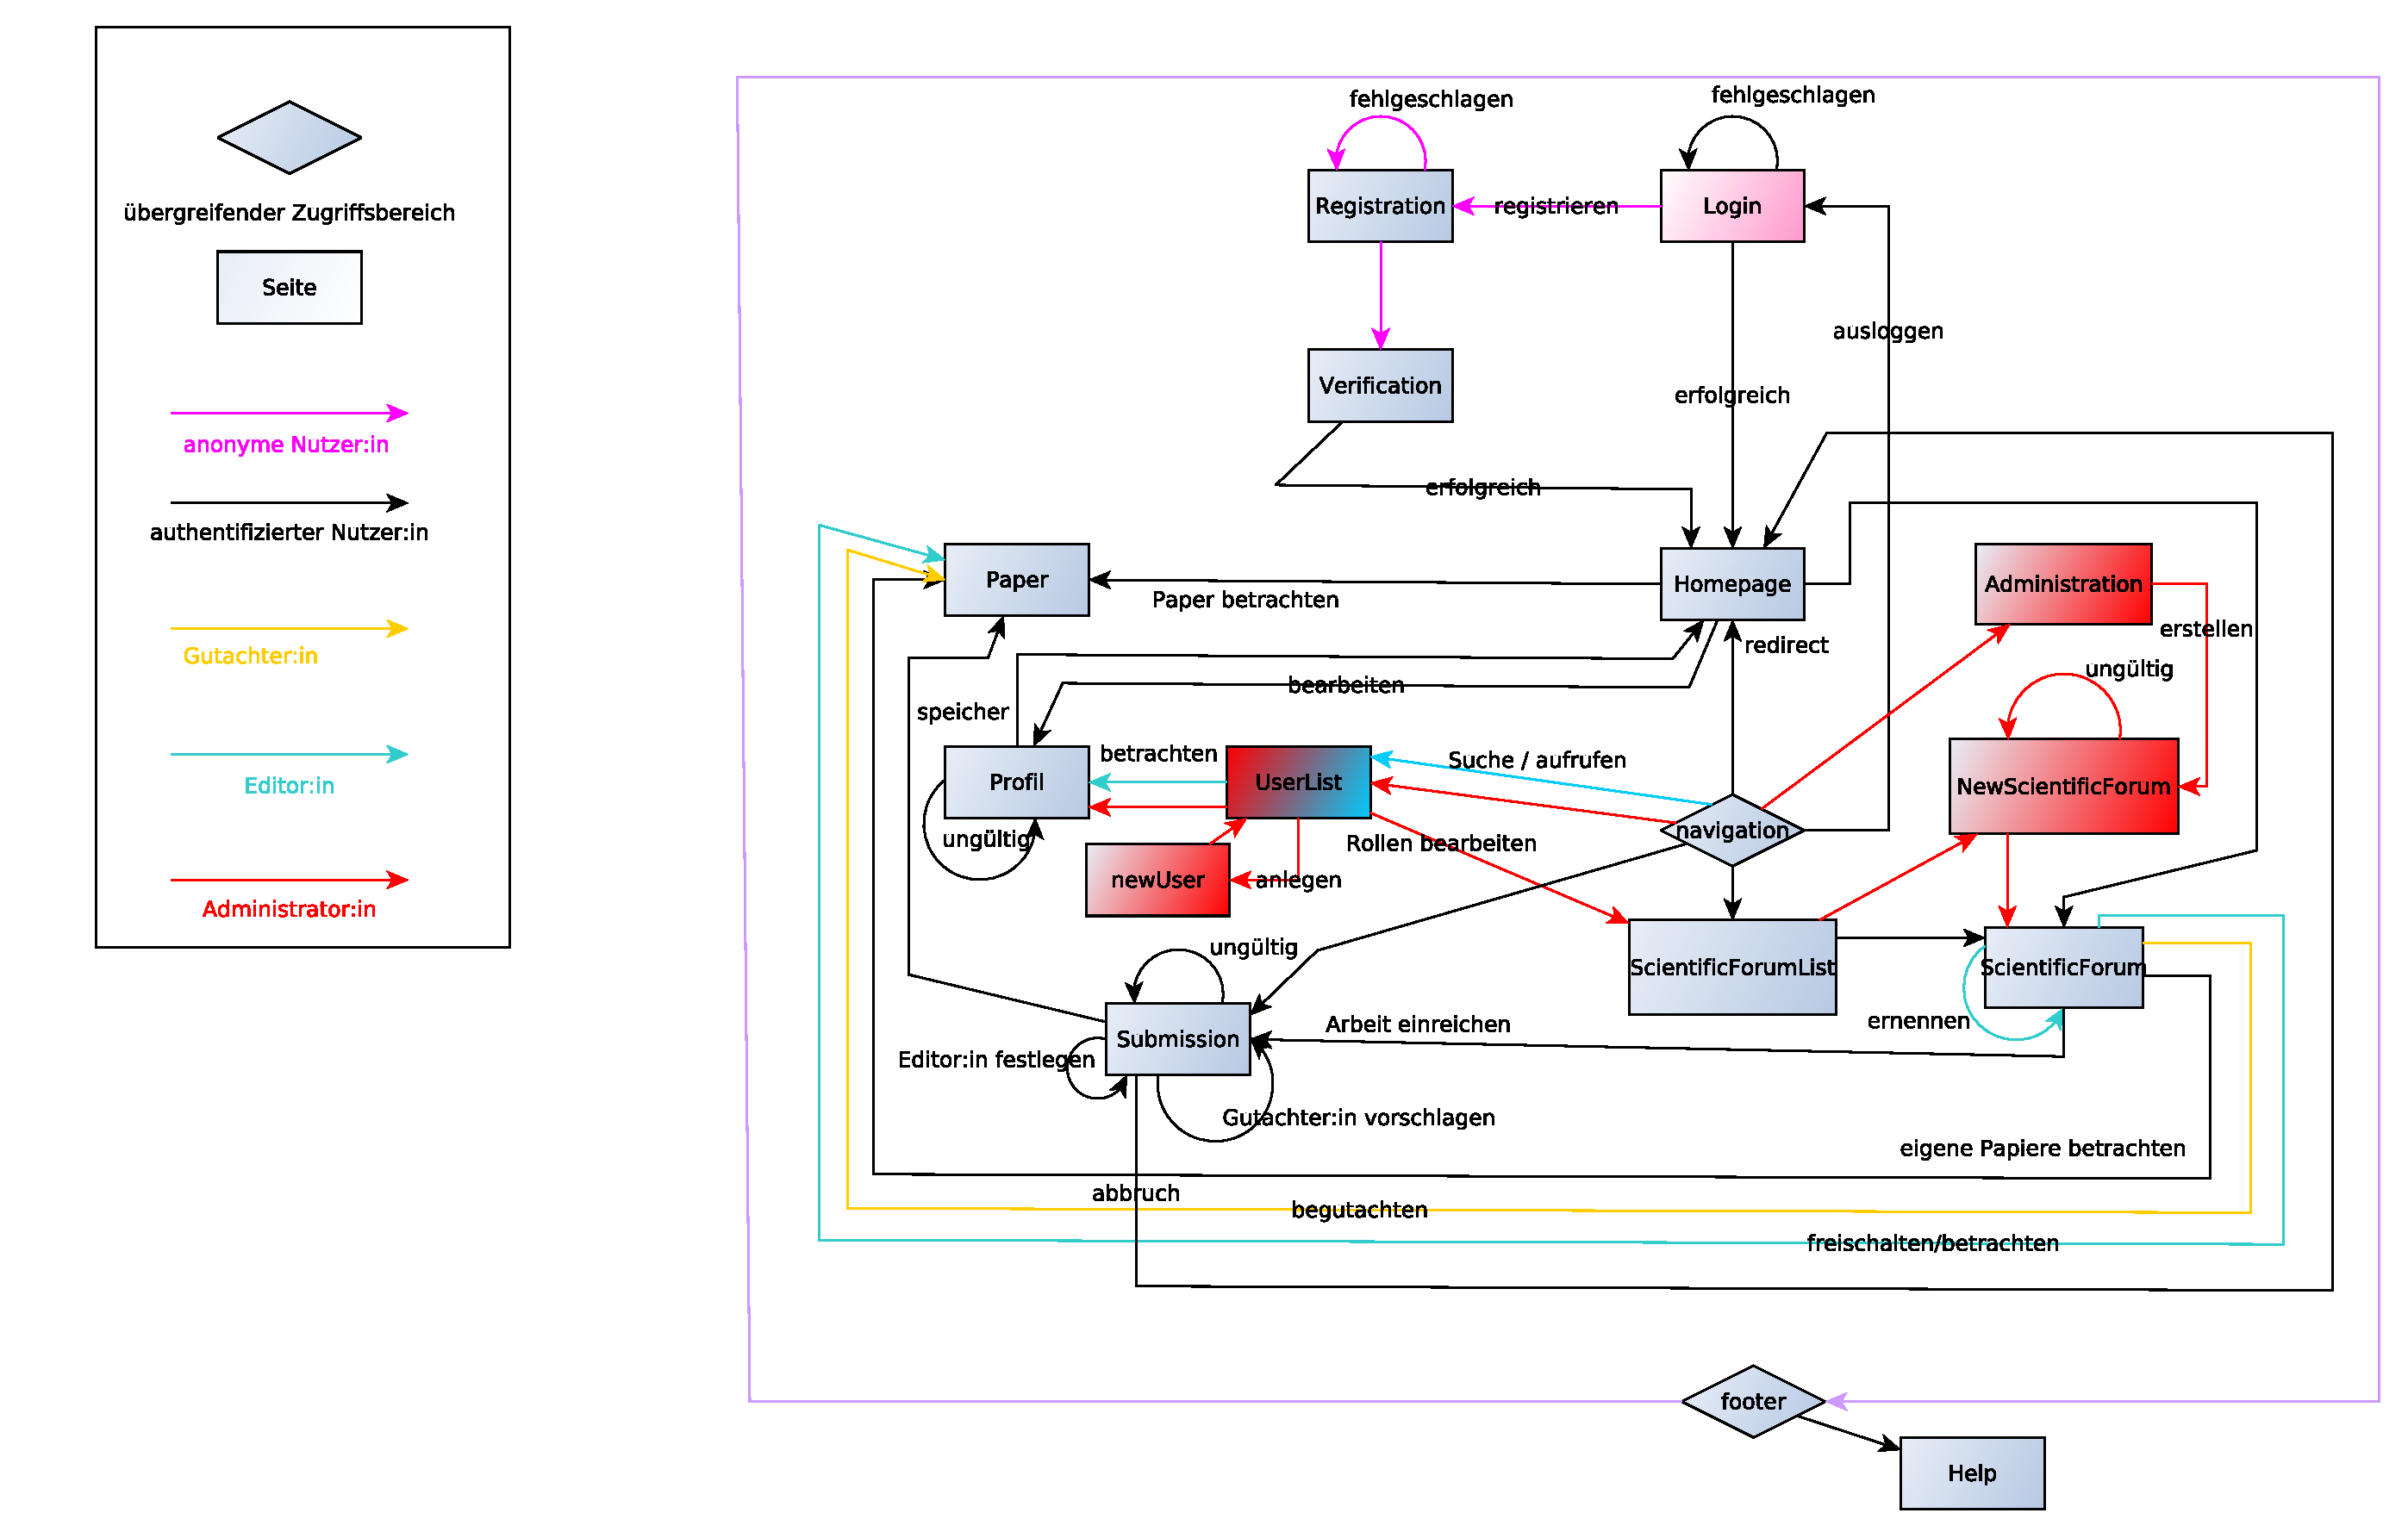
\includegraphics[width=\linewidth]{graphics/benutzerFlussyEd}
    \caption{Benutzerfluss}
\end{figure}

Die sich im Diagramm befindlichen Rauten stellen Header (Navigationsleiste) und Footer dar.
Hierbei wird jedoch wie folgt unterschieden: Der Header ist nur für authentifizierte Nutzer:innen zugänglich,
d.h. dieser erscheint erst nach einem erfolgreichen Login sichtbar und verschwindet nach einem Logout wieder.
Der Footer hingegen ist von jeder Seite der Applikation zugänglich und somit sichtbar.

Im Diagramm werden Administratoren, Editoren, Gutachter und normale Nutzende unter dem allgemeinen Begriff
authentifizierte Nutzer:innen betrachtet.
Sind die Verbindungspfeile nicht schwarz, sondern andersfarbig dargestellt besitzen auch nur die
dargestellten Benutzergruppen ein Zugriffsrecht oder das Recht auf eine Aktion.

Des Weiteren ist der Randfall zu betrachten, bei welchem ein externer Gutachter, welcher noch nicht registriert ist,
eine Einladung eines Editors angenommen hat.
Diesem wird die Rolle eines Gutachters zugewiesen, jedoch besitzt er erst Zugriffsrechte, nachdem er sich
authentifiziert hat.

\subsection{Mockups}

Die Folgenden Bilder zeigen einen Prototypen der Anwendung. Gezeigt sind zwei Ausschnitte aus Schlüsselfunktionen der Webanwendung.

\subsubsection{Homepage}

\begin{figure}[H]
	\centering
	\includegraphics[width=\linewidth]{graphics/Homepage}
	\caption{Übersicht auf der Homepage}
\end{figure}

\subsubsection{Einreichung}

\begin{figure}[H]
	\centering
	\includegraphics[width=\linewidth]{graphics/Paper}
	\caption{Ablauf einer erfolgreichen Einreichung nach Reviews}
\end{figure}

	\section{Qualitätsanforderungen}
	\localauthor{Johann Schicho}

\begin{table}[H]
	\centering
	\begin{tabular}{lccc}
		\toprule
		& zentral & wichtig & nicht im zentralen Fokus \\
		\midrule
		Mehrbenutzerbetrieb & \texttt{x} & & \\
		Robustheit & & \texttt{x} & \\
		Standardkonformität & & \texttt{x} & \\
		Benutzerfreundlichkeit & \texttt{x} & & \\
		Sicherheit & &  \texttt{x} & \\
		Portierbarkeit & & & \texttt{x} \\
		Erweiterbarkeit & & \texttt{x} &  \\
		\bottomrule
	\end{tabular}
\end{table}

	\section{Testfälle}
	\localauthor{Sebastian Vogt}
\todo{Des nummoi erklären mit den TXXX Angelegenheiten}
\subsection{Test Setup}\label{setup}
Vor Ausführung jeglicher Tests sollten folgende Voraussetzungen erfüllt sein:
\begin{itemize}
	\item Das System ist vollständig eingerichtet.
	Insbesondere sind die Datenbankschemata erstellt und die globalen Einstellungen sind getroffen.
	\item Es existiert eine Administratorin mit folgenden Nutzerdaten:
	\begin{itemize}
		\item \emph{E-Mail Adresse}: kirz@fim.uni-passau.de
		\item \emph{Vorname}: Johanna
		\item \emph{Nachname}: Mayer
		\item \emph{Passwort}: UniDorfen1870!
	\end{itemize}
	\item Es existiert ein Nutzer mit folgenden Nutzerdaten:
	\begin{itemize}
		\item \emph{E-Mail Adresse}: schicho@fim.uni-passau.de
		\item \emph{Vorname}: Franz
		\item \emph{Nachname}: Huber
		\item \emph{Passwort}: TSVDorfen2001!
	\end{itemize}
	\item Es existiert eine Nutzerin mit folgenden Nutzerdaten:
	\begin{itemize}
		\item \emph{E-Mail Adresse}: vogt@fim.uni-passau.de
		\item \emph{Vorname}: Petra
		\item \emph{Nachname}: Müller
		\item \emph{Passwort}: TSVDorfen2002!
	\end{itemize}
	\item Es existiert ein Nutzer mit folgenden Nutzerdaten:
	\begin{itemize}
		\item \emph{E-Mail Adresse}: guerster@fim.uni-passau.de
		\item \emph{Vorname}: Tuti
		\item \emph{Nachname}: Aslan
		\item \emph{Passwort}: SupaDöner1970!
	\end{itemize}
\end{itemize}
Die Tests werden in der angegebenen Reihenfolge ausgeführt.
Das heißt jeder Test kann die Zustandsänderungen, die durch vorherige Tests ausgelöst worden sind, als gegeben voraussetzen.
\subsection{Administratoren}
Zuerst testen wir die Funktionen der Administratoren.
Die Einstellungen, die von der Administratorin getroffen werden, können so im Folgenden als Voraussetzungen genutzt werden.
\begin{description}

	\XXitem{/T010/}{t010} \emph{Testet \hyperref[funkt:830]{/F830/}}.
	Die Administratorin meldet sich mit ihren Anmeldedaten im System an und wird zur Startseite weitergeleitet.
	Über die Kopfzeile ruft sie nun die Liste der wissenschaftlichen Foren auf.
	Von dort aus navigiert sie zur Seite zur Erstellung eines neuen wissenschaftlichen Forums.
	Dort erstellt sie ein Forum mit folgenden Daten:
	\begin{itemize}
		\item \emph{Editor:innen}: Nutzer mit E-Mail-Adresse guerster@fim.uni-passau.de
		\item \emph{Name}: Chemie Tagung
		\item \emph{Deadline}: 30.12.2022
		\item \emph{Kurzbeschreibung}: Es geht um Chemie.
		\item \emph{URL}: ch.em.ie
		\item \emph{Anleitung zur Begutachtung}: Begutachten Sie.
	\end{itemize}
	Danach wird sie auf die Seite des wissenschaftlichen Forums weitergeleitet.

	\XXitem{/T015/}{t015} \emph{Testet \hyperref[funkt:830]{/F830/}}.
	Die Administratorin ruft über die Kopfzeile die Liste der wissenschaftlichen Foren auf.
	Von dort aus navigiert sie zur Seite zur Erstellung eines neuen wissenschaftlichen Forums.
	Dort erstellt sie ein Forum mit folgenden Daten:
	\begin{itemize}
		\item \emph{Editor:innen}: Nutzer mit E-Mail-Adresse guerster@fim.uni-passau.de
		\item \emph{Name}: Physik Tagung
		\item \emph{Deadline}: 30.12.2099
		\item \emph{Kurzbeschreibung}: Es geht um Physik.
		\item \emph{URL}: ph.ys.ik
		\item \emph{Anleitung zur Begutachtung}: Begutachten Sie.
	\end{itemize}
	Danach wird sie auf die Seite des wissenschaftlichen Forums weitergeleitet.

\end{description}

\subsection{Angemeldeter Nutzer I}
\begin{description}

	\XXitem{/T020/}{t020} \emph{Testet \hyperref[funkt:160]{/F160/}}.
	Die Nutzerin mit der E-Mail-Adresse vogt@fim.uni-passau.de meldet sich im System an.
	Anschließend gibt sie im Suchfeld in der Kopfzeile ``Chemie Tagung'' ein und schickt die Suchanfrage mit Enter ab.
	Nun wird sie auf die Seite mit den Suchergebnissen weitergeleitet und das Forum namens ``Chemie Tagung'' ist der einzige Eintrag in der angezeigten Liste.
	Nach einem Klick auf diesen Eintrag wird die Nutzerin auf die Seite des wissenschaftlichen Forums weitergeleitet.

	\XXitem{/T030/}{t030} \emph{Testet \hyperref[funkt:400]{/F400/}}.
	Nun navigiert die Nutzerin per Mausklick auf die Seite für eine neue Einreichung.
	dort ist das Feld mit dem wissenschaftlichen Forum bereits richtig ausgefüllt, und zwar mit ``Chemie Tagung''

	\XXitem{/T040/}{t040} \emph{Testet \hyperref[funkt:420]{/F420/}}.
	Anschließend lädt die Nutzerin folgende PDF-Datei hoch: \href{https://dl.acm.org/doi/pdf/10.1145/3321707.3321795}{https://dl.acm.org/doi/pdf/10.1145/3321707.3321795}.

	\XXitem{/T045/}{t045} \emph{Testet \hyperref[funkt:450]{/F450/}}.
	Sie trägt in den Feldern des Formulars folgende Daten ein:
	\begin{itemize}
		\item \emph{Name der Einreichung}: Wichtiges Papier
		\item \emph{Co-Autoren}: Ein Co-Autor mit folgenden Daten:
		\begin{itemize}
			\item \emph{Vorname} Valentin
			\item \emph{Nachname} Kasper
			\item \emph{E-Mail-Adresse} garstenaue
		\end{itemize}
		\item \emph{Editor}: guerster@fim.uni-dorfen.de
	\end{itemize}
	Da die angegebene E-Mail-Adresse nicht gültig ist, ist die Registrierung nicht erfolgreich.
	Sie bleibt auf der Registrierungsseite und wird mit einer Fehlermeldung über das Problem informiert.

	\XXitem{/T050/}{t050} \emph{Testet \hyperref[funkt:410]{/F410/}}.
	Sie trägt wieder die gleichen Daten in das Formular ein wie in Test \hyperref[t050]{/T050/}, nur diesmal mit der E-Mail-Adresse \texttt{garstenaue@fim.uni-passau.de}

	\XXitem{/T060/}{t060} \emph{Testet \hyperref[funkt:460]{/F460/}}.
	Nach erfolgreicher Absendung des Formulars wird die Nutzerin auf die Übersichtsseite der Einreichung weitergeleitet.

	\XXitem{/T070/}{t070} \emph{Testet \hyperref[funkt:460]{/F460/}}.
	Frau Müller ist jetzt fertig mit ihrer Arbeit und führt mit dem zugehörigen Link in der Kopfzeile den Logout durch.
	Sie befindet sich nun wieder auf den Anmeldeseite.
\end{description}

\subsection{Editor I}
\begin{description}

	\XXitem{/T080/}{t080} \emph{Testet \hyperref[funkt:680]{/F680/}}.
	Der Nutzer mit der E-Mail-Adresse guerster@fim.uni-passau.de meldet sich im System an.
	Von der Startseite aus ruft er die Einreichung ``Wichtiges Papier'' auf und landet auf der Seite dieser Einreichung.
	Er gibt in das Formular zur Zuweisung von Gutachtern ``schicho@fim.uni-passau.de'' ein und schickt das Formular ab.
	Anschließend meldet er sich ab.

	\todo{Evenutuell F690, aso die Versendung der Email noch testen...}

	\todo{F700 noch testen, aber nicht hier, sondern nach den Sachen vong Gutachter}

\end{description}

\subsection{Gutachter}
\begin{description}

	\XXitem{/T090/}{t090} \emph{Testet \hyperref[funkt:540]{/F540/}}.
	Der Nutzer mit der E-Mail-Adresse schicho@fim.uni-passau.de meldet sich im System an.
	Von der Startseite aus ruft er die Einreichung ``Wichtiges Papier'' auf und landet auf der Seite dieser Einreichung.
	Er nutzt das angezeigte Formular um eine einseitige PDF-Datei namens \emph{gutachten.pdf} als Gutachten hochzuladen.
	Dann meldet er sich wieder ab mit der Logout Funktionalität.

\end{description}

\subsection{Editor II}
\begin{description}

	\XXitem{/T100/}{t100} \emph{Testet \hyperref[funkt:685]{/F685/}}.
	Der Nutzer guerster@fim.uni-passau.de meldet sich wie oben beschrieben an und navigiert wie oben beschrieben zur Seite der Einreichung ``Wichtiges Papier''.
	Dort sieht er ein Gutachten von schicho@fim.uni-passau.de.
	Er betätigt die Schaltfläche zur Freigabe dieses Gutachtens.
	Dann meldet er sich wieder ab.

\end{description}

\subsection{Anonyme Nutzer}

\begin{description}
	\XXitem{/T200/}{t200} \emph{Testet \hyperref[funkt:010]{/F010/}}. Valentin Kasper aus \hyperref[t050]{/T050/} ist noch nicht im System registriert.
	Er ruft LasEs auf und wird zur Anmeldeseite weitergeleitet.
	\XXitem{/T210/}{t210} \emph{Testet \hyperref[funkt:060]{/F060/}}. Er klickt auf den Link zur Registrierung und gibt seinen Namen, seine E-Mail-Adresse und das Passwort \texttt{einsZwei3!5678} an.

	Die Registrierung wird bestätigt und er erhält eine Verifizierungs-E-Mail.
	\XXitem{/T220/}{t220} \emph{Testet \hyperref[funkt:070]{/F070/}}. Er klickt auf den Bestätigungslink in der E-Mail und wird auf die Verifizierungsseite weitergeleitet.
	Damit ist sein Profil erstellt.
	Er wird automatisch auf die Homepage weitergeleitet.
	\XXitem{/T230/}{t230} \emph{Testet \hyperref[funkt:260]{/F260/}}. Da er als Ko-Autor in Test \hyperref[t050]{/T050/} eingetragen wurde, wird ihm das Paper auf der Homepage angezeigt. Der Nutzer meldet sich ab.
\end{description}

\subsection{Angemeldeter Nutzer II}

\begin{description}

	\XXitem{/T110/}{t110} \emph{Testet \hyperref[funkt:480]{/F480/}}.
	Nun meldet sich die Nutzerin vogt@fim.uni-passau.de an und navigiert zur Seite der Einreichung ``Wichtiges Papier''.
	Dort ist das Gutachten von schicho@fim.uni-passau.de sichtbar.
	Nach Betätigung der Download Schaltfläche wird die PDF-Datei \emph{gutachten.pdf} vom Browser heruntergeladen.

	\XXitem{/T120/}{t120} \emph{Testet \hyperref[funkt:230]{/F230/}}.
	Auf der Navigationsleiste klickt die Nutzerin nun den Link, der zum Profil führt.
	Die Profil-Seite wird angezeigt.
	Die Nutzerin betätigt nun die Schaltfläche zur Löschung des Kontos.
	Daraufhin wird eine Warnung angezeigt, dass dies sowohl alle Einreichungen löscht, als auch die Editoren und Gutachter der eingereichten Paper per E-Mail benachrichtigt.
	Die Nutzerin akzeptiert diese Nachricht und wird auf die Anmeldeseite weitergeleitet.
	Der Nutzer schicho@fim.uni-passau.de hat nun eine E-Mail über die Löschung des Nutzers erhalten.
	Er meldet sich wieder ab.
	Die Administratorin meldet sich nun im System an, navigiert über die Navigationsleiste zur Liste der wissenschaftlichen Foren und von dort auf auf ``Chemie Tagung''. Dort stellt er fest, dass keine Paper existieren.

\end{description}

\subsection{Reset}
Der Programmzustand, der im Abschnitt \emph{\hyperref[setup]{Setup}} beschrieben ist, muss nach den Tests wiederhergestellt werden.
Dies ermöglicht eine weitere korrekte Durchführung der Tests.





	\section{Entwicklungsumgebung}
	\localauthor{Sebastian Vogt}
\subsection{Programmierung}
\begin{itemize}
	\item \textbf{Betriebssystem}: Die Entwickler verwenden Windows 10, Windows 11 und Ubuntu 20.04
	\item \textbf{IDE \todo{Glossar}}: JetBrains IntelliJ
	\item \textbf{Build Tool \todo{Glossar}}: Apache Maven
\end{itemize}
\subsection{Referenzumgebung}
\begin{itemize}
	\item \textbf{Webserver \todo{Glossar}}: Tomcat 10.0.10
	\item \textbf{Betriebssystem}: Debian 11
	\item \textbf{Deployment \todo{Glossar}}: Das Projekt wird durch das \textbf{WAR Plugin in Maven} als \textbf{WAR Datei \todo{Glossar}} exportiert. Diese Datei wird dann von Tomcat zum Zugriff zur Verfügung gestellt.
\end{itemize}
\subsection{Versionskontrolle}
\begin{itemize}
	\item \textbf{Git} Version 2.25.1
	\item \textbf{Zusammenarbeit} im Team wird über den \textbf{GitLab \todo{Glossar}} Server der Fakultät für Informatik und Mathematik der Universität Passau gehandhabt.
\end{itemize}
\subsection{Dokumente}
\begin{itemize}
	\item \textbf{LaTex Compiler \todo{Glossar}}: LuaHBTeX, Version 1.13.2
	\item \textbf{LaTex Distribution \todo{Glossar}}: TeX Live 2021
\end{itemize}
\subsection{Diagramme}
\begin{itemize}
	\item \textbf{Klassendiagramm \todo{Glossar}}: IBM Rational Software Architect auf Debian 11
	\todo{Die Programme, die wir für Diagramme verwenden noch ergänzen.}
\end{itemize}

	\section{Glossar}
	\localauthor{Stefanie Gürster}

\begin{description}
	\XXitem{Build Tool}{glo:buildtool} Apache Maven ist ein Build System für Java Anwendungen. Es erlaubt die einfache Einbindung von weiteren Softwarebibliotheken und übernimmt den Bau eines \hyperref[glo:war]{\texttt{war}} Archivs.

	\XXitem{GitLab}{glo:gitlab} GitLab ist ein zentraler Speicherplatz für alle Entwickler. Darüber kann die Zusammenfügung einzelner Codestücke verwaltet werden.

	\XXitem{Gutachter}{glo:gutachter} Gutachter:innen können anonym die Paper anderer Wissenschaftler \emph{peer-reviewen} und Änderungen verlangen oder es als gut befinden.

	\XXitem{IBM RSA}{glo:rsa} Der \emph{IBM Rational Software Architect} erlaubt \emph{Round-Trip Engineering}. Damit können gleichzeitig zur Programmierung auch die aus dem Code hervorgehenden Diagramme erstellt werden.

	\XXitem{Inkscape}{glo:inkscape} Inkscape ist ein Vektorgrafikbearbeitungsprogramm. Vektorgrafiken haben den Vorteil bei nahem \emph{heranzoomen} nicht unscharf zu werden.

	\XXitem{In-Memory Datenbank}{glo:ramdb} Zur vereinfachten Entwicklung wird während der Entwicklungsphase nicht eine echte Datenbank mit hoher Latenzzeit verwendet, sondern eine lokale Arbeitsspeicher Datenbank.

	\XXitem{IDE}{glo:ide} \emph{Integrated Development Environment} Programm, in der die Webanwendung programmiert wird und bei der Entwicklungsarbeit unterstützt.

	\XXitem{JDK}{glo:jdk} \emph{Java Development Kit} Komplette Softwarebibliothek der Java Programmiersprache. Enthält die Grundbausteine der Anwendung.

	\XXitem{Journal}{glo:journal} Zu einer Konferenz kann ein Wissenschaftler ein Manuskript in Form eines PDFs abgeben. Ein Journal hat keine Deadline zur Abgabe.

	\XXitem{Konferenz}{glo:konf} Zu einer Konferenz kann ein Wissenschaftler ein Manuskript in Form eines PDFs abgeben. Eine Konferenz hat eine Deadline zur Abgabe.

	\XXitem{\LaTeX}{glo:latex} Latex ist das Textsatzsystem zum verfassen der Dokumente. Es ermöglicht die parallele Bearbeitung von Textdokumenten.

	\XXitem{Submission}{glo:submission} Eine \emph{Einreichung} ist das hochladen eines Manuskripts auf den Datenbankserver durch den veröffentlichenden Wissenschaftler:in. Anschließend können Gutachter:innen dieses Manuskript reviewen.

	\XXitem{war}{glo:war} \emph{Web Application Resource} oder \emph{Web Archive} Archivdateiformat. Bündelt die Anwendung in eine einzige Datei, die damit leicht installierbar ist.

	\XXitem{yEd}{glo:yed} Bearbeitungsprogramm zum erstellen von Graphen und Diagrammen.
\end{description}


<<<<<<< HEAD
\end{document}
=======
\end{document}
>>>>>>> df2db1ff87a04e7e122cc20cf738e10e37059346
